% ********** Chapter 7 **********
\chapter{Analyse}
\label{sec:Hoofdstuk 7}

In dit hoofdstuk zullen de verschillende datastructuren vergeleken worden. Dit zal gebeuren aan de hand van de aangeleverde tekst bestanden.

Deze benchmarks zijn genomen van een systeem eigendom van de Rijksuniversiteit Groningen. De specificaties waren:

\begin{enumerate}
  \item Intel Core 2 Duo CPU (E6550 @ 2.33 GHz)
	\item 2 Gigabyte RAM geheugen
	\item GNU/Linux besturingssysteem kernel 2.6.32 (i686)
\end{enumerate}

\section{Tekstbestand 1}

Dit bestand bestaat uit 18.336 woorden, die in alfabetische volgorde gesorteerd staan. De verwachting is dat de normale ongebalanceerde binaire boom hier erg slecht presteert, dit omdat een 'worst case' binaire boom oplevert. Alle nodes zullen aan een kant van de boom zitten.

Het gemiddelde van 10 epochs (aantal tests) van het opbouwen van de structuren is opgenomen in tabel \ref{tbl_text1_build}, de resultaten voor het opzoeken staan in tabel \ref{tabel}.

\begin{table}
\begin{tabularx}{\linewidth}{| l | X| X| X | }
 \hline
Structuur & String vergelijkingen &  Toekenningen & Run time \\
 \hline
 	Binaire Boom & 336.190.560 & 672.491.133 & 4729 ms. \\
 	\hline
 	AVL Boom & 242.273 & 1.304.131 & 12,5 ms \\
 	\hline
 	Skip List & 515.116,5 & 1.084.854,2 & 19,1 ms \\
 	\hline
 	(2,4)-Boom & 647.141 & 1.169.220 & 48,4 ms \\
 	\hline
\end{tabularx}
\label{tbl_text1_build}
\caption{Opbouwen van text 1}
\end{table}

\begin{table}
\begin{tabularx}{\linewidth}{| l | X| X| X | }
 \hline
 Structuur & String vergelijkingen &  Toekenningen & Run time \\
 \hline
 	Binaire Boom & 168.113.616 & 336.227.232 & 2282,3 ms. \\
 	\hline
 	AVL Boom & 242.288 & 818.544 & 7,4 ms \\
 	\hline
 	Skip List & 512.749,2 & 531.085,2 & 11 ms \\
 	\hline
 	(2,4)-Boom & 574.193 & 429.481 & 22,2 ms \\
 	\hline
\end{tabularx}
\label{tbl_text1_search}
\caption{Doorzoeken van text 1}
\end{table}

De waarden voor de datastructuren (met uitzondering van de binaire boom) zijn geplot in figuur \ref{fig:opbouwtext1} en \ref{fig:zoektext1}.

\begin{figure}[h]
	\centering
		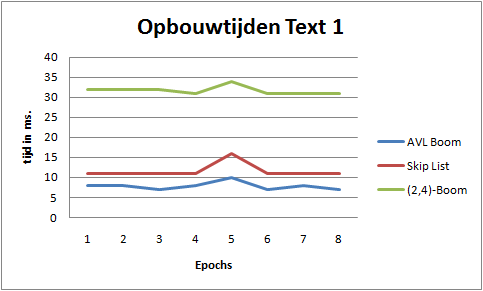
\includegraphics[width=\textwidth]{chap7/opbouwtijdtext1}
		\caption{De opbouwtijden van bestand text1.}
	\label{fig:opbouwtext1}
\end{figure}

\begin{figure}[h]
	\centering
		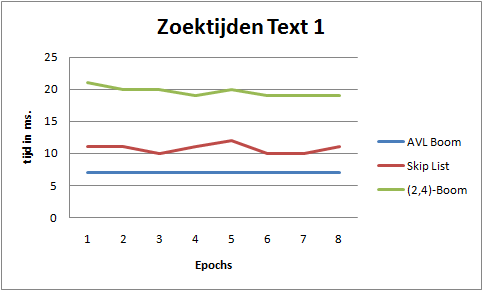
\includegraphics[width=\textwidth]{chap7/zoektijdtext1}
		\caption{De doorzoek tijden van bestand text1.}
	\label{fig:zoektext1}
\end{figure}

\clearpage

\section{Tekstbestand 2}

Dit tekst bestand is hetzelfde als Textbestand 1, alleen is nu de alfabetische sortering omgedraait. Voor de normale binaire boom betekend dit dat de boom in principe omgekeerd is, dit is ook een 'worst case' voor de binaire boom.

\begin{table}
\begin{tabularx}{\linewidth}{| l | X| X| X | }
 \hline
 Structuur & String vergelijkingen &  Toekenningen & Run time \\
 \hline
 	Binaire Boom & 336.190.560 & 672.491.133 & 5.649,3 ms. \\
 	\hline
 	AVL Boom & 242.273 & 1.304.131 & 13,4 ms. \\
 	\hline
 	Skip List & 290.419,8 & 841.339,8 & 9,5 ms. \\
 	\hline
 	(2,4)-Boom & 1150025 & 1251704 & 62.3 ms. \\
 	\hline
\end{tabularx}
\label{tbl_text1_search}
\caption{Opbouw tijden van de datastructuren}
\end{table}


\begin{table}
\begin{tabularx}{\linewidth}{| l | X| X| X | }
 \hline
 Structuur & String vergelijkingen &  Toekenningen & Run time \\
 \hline
 	Binaire Boom &168.113.616 & 336.227.232 &  2977,1 ms. \\
 	\hline
 	AVL Boom &242.288
 & 818.544 & 6,7
 ms \\
 	\hline
 	Skip List &535.087,5
 & 553.423,5
 &  10,9 ms \\
 	\hline
 	(2,4)-Boom &524.697 & 532.957 &  26,5 ms \\
 	\hline
\end{tabularx}
\label{tbl_text1_search}
\caption{Zoek tijden voor de datastructuren}
\end{table}

De gemiddelde tijden van de datastructuren zijn geplot in figuur \ref{fig:opbouwtext2} en \ref{fig:zoektext2}.


\begin{figure}[h]
	\centering
		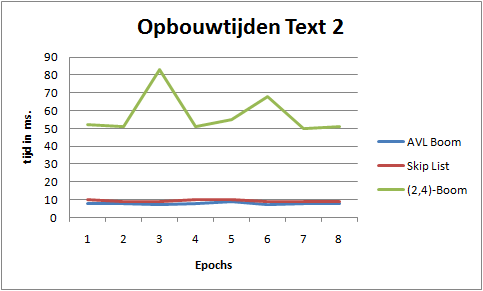
\includegraphics[width=\textwidth]{chap7/opbouwtijdtext2}
		\caption{De opbouwtijden van bestand text2.}
	\label{fig:opbouwtext2}
\end{figure}

\begin{figure}[h]
	\centering
		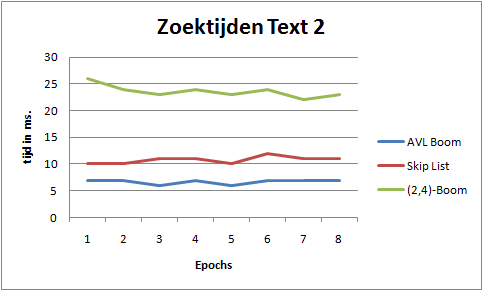
\includegraphics[width=\textwidth]{chap7/zoektijdtext2}
		\caption{De opbouwtijden van bestand text2.}
	\label{fig:zoektext2}
\end{figure}

\clearpage

\section{Tekstbestand 3}

Dit tekst bestand bestaat uit 18.336 woorden, alleen zijn deze nu niet gesorteerd. Wat opvalt is dat de binaire boom in dit geval erg goed presteert.

\begin{table}
\begin{tabularx}{\linewidth}{| l | X| X| X | }
 \hline
 Structuur & String vergelijkingen &  Toekenningen & Run time \\
 \hline
 	Binaire Boom & 613.660 & 1.337.333 & 19,7 ms. \\
 	\hline
 	AVL Boom & 237.809 & 1.184.931 & 16,5  ms. \\
 	\hline
 	Skip List & 487.298,7 & 1.056.974 & 20,9 ms. \\
 	\hline
 	(2,4)-Boom & 698.519 & 1.021.189 & 58,7 ms. \\
 	\hline
\end{tabularx}
\label{tbl_text1_search}
\caption{Opbouwtijden data structuren text 3.}
\end{table}


\begin{table}
\begin{tabularx}{\linewidth}{| l | X| X| X | }
 \hline
 Structuur & String vergelijkingen &  Toekenningen & Run time \\
 \hline
 	Binaire Boom & 325.166 & 650.332 & 10,4 ms. \\
 	\hline
 	AVL Boom & 246.521 & 831.243 & 10,5 ms. \\
 	\hline
 	Skip List & 509.393,3 & 527.729,3 & 18,6 ms. \\
 	\hline
 	(2,4)-Boom & 622.921 & 431.363 & 31,1 ms. \\
 	\hline
\end{tabularx}
\label{tbl_text1_search}
\caption{Zoek tijden datastructuren text 3}
\end{table}

\begin{figure}[h]
	\centering
		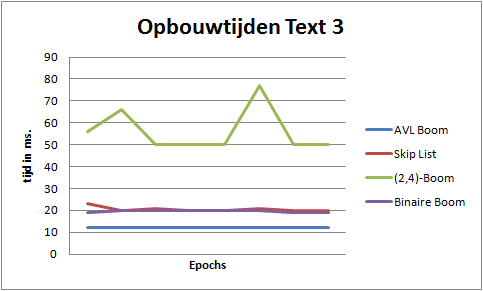
\includegraphics[width=\textwidth]{chap7/opbouwtijdtext3}
		\caption{De opbouwtijden van bestand text3.}
	\label{fig:opbouwtext3}
\end{figure}

\begin{figure}[h]
	\centering
		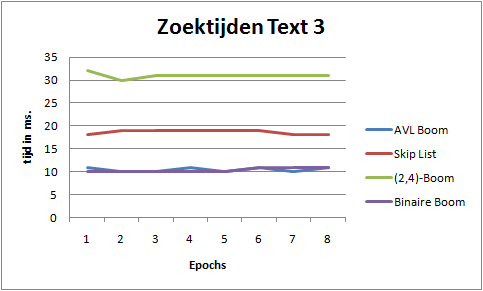
\includegraphics[width=\textwidth]{chap7/zoektijdtext3}
		\caption{De opbouwtijden van bestand text3.}
	\label{fig:zoektext3}
\end{figure}


\clearpage

\section{Tekstbestand 4}

Dit tekst bestand bestaat uit 38.375 woorden, dit tekst bestand is ook alfabetisch gesorteerd. De binaire boom is weer in een 'worst case' terecht gekomen, en dit is te zien aan de executie tijd.

\begin{table}
\begin{tabularx}{\linewidth}{| l | X| X| X | }
 \hline
 Structuur & String vergelijkingen &  Toekenningen & Run time \\
 \hline
 	Binaire Boom & 1.472.602.250& 2.945.434.747  & 20.423,4 ms. \\
 	\hline
 	AVL Boom & 548.465 & 2.853.906 & 22,4 ms \\
 	\hline
 	Skip List & 1.145.175,4 & 2.334.426,8 & 24,5  ms \\
 	\hline
 	(2,4)-Boom & 1.456.303 & 2.548.444 & 80,2 ms \\
 	\hline
\end{tabularx}
\label{tbl_text1_search}
\caption{caption}
\end{table}


\begin{table}
\begin{tabularx}{\linewidth}{| l | X| X| X | }
 \hline
 Structuur & String vergelijkingen &  Toekenningen & Run time \\
 \hline
 	Binaire Boom & 736.339.500 & 1.472.679.000 & 9.829,4 ms. \\
 	\hline
 	AVL Boom & 548.481 & 1.837.318  & 15,6 ms. \\
 	\hline
 	Skip List & 1.169.080,3& 1.207.455,3 &  23,4 ms. \\
 	\hline
 	(2,4)-Boom & 1.282.218 & 994.303 & 48,1 ms. \\
 	\hline
\end{tabularx}
\label{tbl_text1_search}
\caption{caption}
\end{table}


\begin{figure}[h]
	\centering
		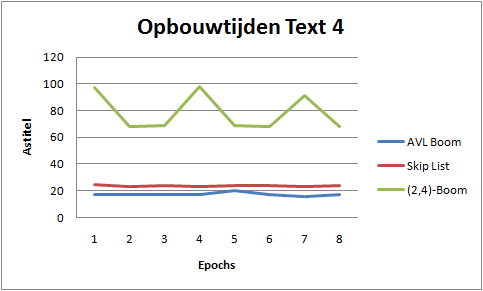
\includegraphics[width=\textwidth]{chap7/opbouwtijdtext4}
		\caption{De opbouwtijden van bestand text4.}
	\label{fig:opbouwtext4}
\end{figure}

\begin{figure}[h]
	\centering
		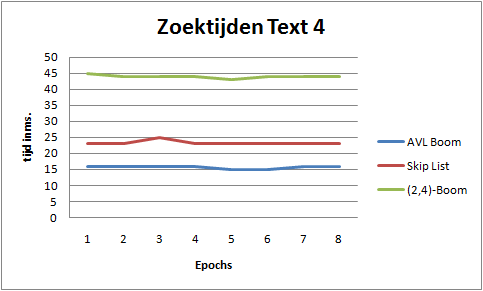
\includegraphics[width=\textwidth]{chap7/zoektijdtext4}
		\caption{De opbouwtijden van bestand text4.}
	\label{fig:zoektext4}
\end{figure}


\clearpage

\section{Tekstbestand 5}

Dit bestaat uit 191.875 dubbele woorden, in willekeurige volgorde. Ook hier functioneert de normale binaire boom heel snel.

\begin{table}
\begin{tabularx}{\linewidth}{| l | X| X| X | }
 \hline
 Structuur & String vergelijkingen &  Toekenningen & Run time \\
 \hline
 	Binaire Boom &4.257.080

 & 8.897.907 & 159,3
 ms. \\
 	\hline
 	AVL Boom &2.773.238

 & 10.227.649 & 156,9 ms. \\
 	\hline
 	Skip List & 6.111.963,7
& 7.302.252,4
 & 318,8
 ms. \\
 	\hline
 	(2,4)-Boom & 7.436.395
& 6.424.654
 & 542,8
 ms \\
 	\hline
\end{tabularx}
\label{tbl_text4_search}
\caption{Doorzoek tijden text 4}
\end{table}


\begin{table}
\begin{tabularx}{\linewidth}{| l | X| X| X | }
 \hline
 Structuur & String vergelijkingen &  Toekenningen & Run time \\
 \hline
 	Binaire Boom & 3.611.525
&  7.223.050
& 135,9
 ms. \\
 	\hline
 	AVL Boom & 2.791.420
& 9.333.635

 & 151,9
 ms \\
 	\hline
 	Skip List &6.042.471,5
 & 6.234.346,5
& 313,7
 ms \\
 	\hline
 	(2,4)-Boom & 7.024.950
&  5.063.905
&  432
ms. \\
 	\hline
\end{tabularx}
\label{tbl_text1_search}
\caption{caption}
\end{table}


\begin{figure}[h]
	\centering
		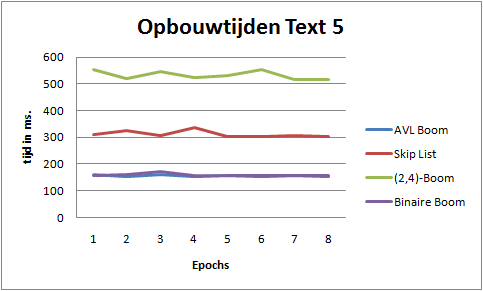
\includegraphics[width=\textwidth]{chap7/opbouwtijdtext5}
		\caption{De opbouwtijden van bestand text5.}
	\label{fig:opbouwtext5}
\end{figure}

\begin{figure}[h]
	\centering
		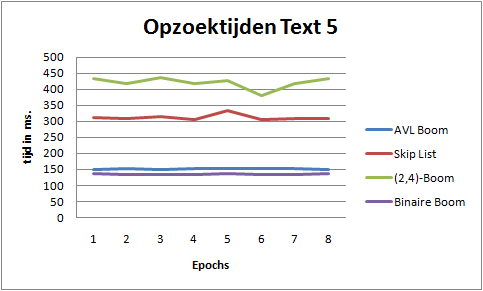
\includegraphics[width=\textwidth]{chap7/zoektijdtext5}
		\caption{De opbouwtijden van bestand text5.}
	\label{fig:zoektext5}
\end{figure}

% ********** End of chapter **********